\documentclass[12pt,utf8]{beamer}

% Gute Einführung zu LaTeX-Beamer: http://www2.informatik.hu-berlin.de/~mischulz/beamer.html

%-----PARAMETERS-----

%Wichtige Standard Pakete!
%\usepackage[german]{babel}
\usepackage{ngerman}
\usepackage{xcolor}
\usepackage{graphicx}
\usepackage{tikz}

%Für den Header notwendig!
%\usepackage[percent]{overpic}

\usepackage{hyperref} % für korrekte Links

%Einbinden des Themes
\input{design_latex-template/beamerthemeFOSSAG.sty}


%Standard Angaben
\title{
	\hspace*{8cm}
	
\includegraphics[scale=0.2]{resources/logo_500px.png}
	\newline
	FOSS-AG
}
\subtitle{Tensorflow - Workshop}
%\author{@chef\_excellence}
\institute[FOSS AG]{\textbf{F}ree and \textbf{O}pen \textbf{S}ource \textbf{S}oftware \textbf{AG}}

\date{29. Mai 2018}

%-----IMPLEMENTATION-----
\begin{document}
	\begin{frame}
		\titlepage
	\end{frame}

	\begin{frame}
		\centering Was ist Machine Learning?
	\end{frame}

	\begin{frame}
		\centering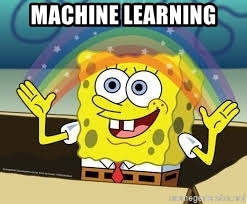
\includegraphics[scale=1]{resources/machine-learning.jpg}\\
		{\tiny Source: \cite{memegen}}
	\end{frame}

	\begin{frame}
		\frametitle{Was ist Machine Learning?}
		\begin{itemize}
			\item Lernen/Schätzen von Eigenschaft eines Datensatzes mittels statistischer Verfahren
			\item Generalisierung von Lerndaten auf Gesamtmenge
		\end{itemize}
	\end{frame}
	
	\begin{frame}
		\frametitle{Machine Learning - Probleme}
		\begin{itemize}
			\item Klassifikation / Clustering
			\item Regression
			\item Prognosen / Vorhersagen
			\item Synthese
		\end{itemize}
	\end{frame}
	
	\begin{frame}
		\frametitle{Machine Learning - Probleme}
		\begin{itemize}
			\item Klassifikation / Clustering
			\item \textcolor{black!20}{Regression}
			\item\textcolor{black!20}{Prognosen / Vorhersagen}
			\item \textcolor{black!20}{Synthese}
		\end{itemize}
	\end{frame}
	
	\begin{frame}
		\frametitle{Machine Learning - Modelle}
		\begin{itemize}
			\item Support Vector Machines
			\item Artificial Neural Networks
			\item Random Markov Fields
			\item k-Nearest Neighbors
		\end{itemize}
	\end{frame}	
	
	\begin{frame}
		\frametitle{Machine Learning - Modelle}
		\begin{itemize}
			\item \textcolor{black!20}{Support Vector Machines}
			\item Artificial Neural Networks
			\item \textcolor{black!20}{Random Markov Fields}
			\item \textcolor{black!20}{k-Nearest Neighbors}
		\end{itemize}
	\end{frame}
	
	\begin{frame}
		\frametitle{Artificial Neural Networks}
		\begin{figure}[h]
			\def\layersep{2.5cm}
			\centering
			\begin{tikzpicture}[shorten >=1pt,->,draw=black!50, node distance=\layersep]
			\tikzstyle{every pin edge}=[<-,shorten <=1pt]
			\tikzstyle{neuron}=[circle,draw,minimum size=17pt,inner sep=0pt]
			\tikzstyle{input neuron}=[neuron];
			\tikzstyle{output neuron}=[neuron];
			\tikzstyle{hidden neuron}=[neuron];
			\tikzstyle{annot} = [text width=4em, text centered]
			
			% Draw the input layer nodes
			\foreach \name / \y in {1,...,4}
			% This is the same as writing \foreach \name / \y in {1/1,2/2,3/3,4/4}
			\node[input neuron, pin=left:$x_\y$] (I-\name) at (0,-\y) {};, the bias allows us to shift the activation function (see below) to the left or right.
			
			% Draw the hidden layer nodes
			\foreach \name / \y in {1,...,5}
			\path[yshift=0.5cm]
			node[hidden neuron] (H-\name) at (\layersep,-\y cm) {};
			
			% Draw the output layer node
			\node[output neuron,pin={[pin edge={->}]right:$y$}, right of=H-3] (O) {};
			
			% Connect every node in the input layer with every node in the
			% hidden layer.
			\foreach \source in {1,...,4}
			\foreach \dest in {1,...,5}
			\path (I-\source) edge (H-\dest);
			
			% Connect every node in the hidden layer with the output layer
			\foreach \source in {1,...,5}
			\path (H-\source) edge (O);
			
			% Annotate the layers
			\node[annot,above of=H-1, node distance=1cm] (hl) {Hidden layer};
			\node[annot,left of=hl] {Input layer};
			\node[annot,right of=hl] {Output layer};
			\end{tikzpicture}
		\end{figure}
	\end{frame}
	
	\begin{frame}
		\frametitle{Artificial Neural Networks}
		\begin{figure}[h]
			\centering
			\begin{tikzpicture}
			\tikzstyle{value} = []
			\tikzstyle{neuron}=[circle,draw, minimum size=25pt,inner sep=0pt]
			\tikzset{edge/.style = {->,> = latex}}
			
			\node[value](x) at (-2,0) {$x$};
			\node[neuron](1) at (0,0) {};
			\node[value](y) at (2,0) {$y$};
			\node[value](b) at (0,1.5) {$b$};
			
			\draw[edge] (x) --node [above] {$W$} (1);
			\draw[edge] (b) to (1);
			\draw[edge] (1) to (y);					
			\end{tikzpicture}
		\end{figure}
		\centering $y = f(x) = h(Wx + b)$
	\end{frame}
	
	\begin{frame}
		\frametitle{Artificial Neural Networks}
		\begin{center}
			$y = f(x) = h(Wx + b)$
		\end{center}
		\begin{itemize}
			\item $x$ - Eingabe
			\item $y$ - Ausgabe
			\item $W$ - Gewichtung
			\item $b$ - Korrekturfaktor
			\item $h$ - Aktivierungsfunktion
		\end{itemize}
	\end{frame}
	
	\begin{frame}
		\frametitle{Artificial Neural Networks}
		\begin{itemize}
			\item zufällige Werte als Eingabe ziehen
			\item Ausgabe berechnen
			\item Ausgabe mit Label vergleichen
			\item Fehlerwert (loss) berechnen
			\item Gewichte anpassen, sodass Fehlerwert minimiert wird
		\end{itemize}
	\end{frame}
	
	\begin{frame}
		\frametitle{Artificial Neural Networks}
		\centering \url{http://playground.tensorflow.org}
		% ex1 data = 2, 2in0h, 0.1, lin
		% ex2 data = 3, 2in3h, 0.1, sig
	\end{frame}
	
	\begin{frame}
		\bibliographystyle{plain}
		\bibliography{literatur}
		\addcontentsline{toc}{section}{\bibname}
	\end{frame}

\end{document}
